\documentclass{article}
\usepackage[utf8]{inputenc}
\usepackage{amsmath, amssymb, amsthm}
\usepackage[shortlabels]{enumitem}
\usepackage{graphicx} % Required for inserting images

\title{MATH512 - Project 2}
\author{Wasif Ahmed, Haoxiang Deng, Jacob Fein-Ashley, Kanav Malhotra}
\date{February 2024}

\begin{document}

\maketitle

\section*{Question 1}
\begin{enumerate}[(a)]
    \item 
        We set up a hypothesis test to determine if the data is uniformly distributed. We use
        the Kolmogorov-Smirnov test to test the null hypothesis that the data is uniformly
        distributed. The test statistic is given by
        \[
            D = \max_{1 \leq i \leq n} \left\{ \frac{i}{n} - F(X_{(i)}) \right\}
        \]
        where $F(X_{(i)})$ is the empirical distribution function of the data. We then compare
        the test statistic to the critical value of the Kolmogorov-Smirnov distribution to
        determine if we can reject the null hypothesis. We use a significance level of $\alpha = 0.05$.

        We find that the test statistic is $D = 0.010$ and a $p$-value of $0.20$. Since the $p$-value
        is greater than the significance level, we fail to reject the null hypothesis. Thus, we
        conclude that the data is uniformly distributed. Note the histogram provided below. 
        It appears that the data is uniformly distributed.\\
        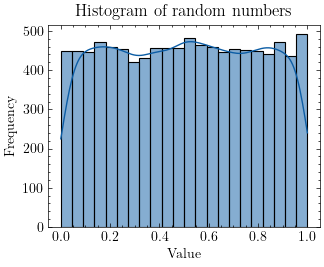
\includegraphics[scale=0.7]{imgs/1a.png}

    \item
        For the first set of parameters, we notice that the data starts at $x_0 = 3$ and then
        generates $[ 3.  7.  9. 10.  5.  8.  4.  2.  1.  6.]$ for $n = 10$. The period is $11$.
        For the second set of parameters, we notice that
        the data starts at $x_0 = 3$ and then stays at $x_n = 8$ for the rest of the data. The sequence is 
        $[3. 8. 8. 8. 8. 8. 8. 8. 8. 8.]$. This is not a random sequence and is not uniformly distributed.
        The period is $5$.

    \item
        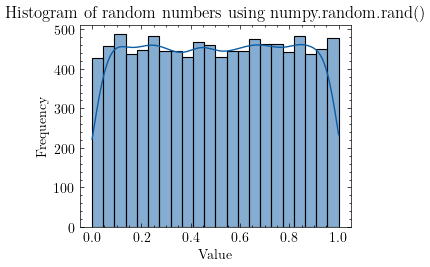
\includegraphics[scale=0.7]{imgs/1d.png} \\ 
        The histogram of the data generated by the linear congruential generator with the first set of parameters
        appears to be uniformly distributed, and quite similar to the histogram of the data generated by the
        numpy random number generator. 

    \item
        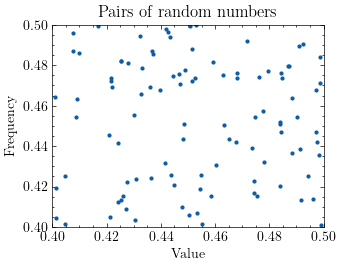
\includegraphics[scale=0.7]{imgs/pairs.png} \\
        I'm not seeing a pattern...

    \item
        We notice that a downfall of the linear congruential generator is that it can appear to be random with the
        right set of parameters, but as we saw with the second parameters in part $b$, the data can be very non-random.
        This is a problem because we want to be able to trust the data that we generate.
\end{enumerate}

\section*{Question 2}
\begin{enumerate}[(a)]
    \item 
        \begin{verbatim}
            x = np.random.rand(10000)
            y = np.zeros(10000)
            y[x < 0.3] = 1
            y[(x >= 0.3) & (x < 0.5)] = 2
            y[(x >= 0.5) & (x < 0.85)] = 3
            y[(x >= 0.85)] = 4
        \end{verbatim}

    \item
        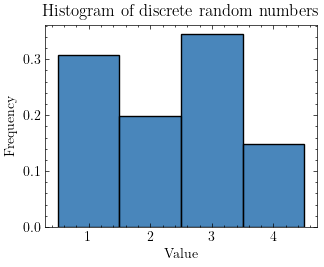
\includegraphics[scale=0.7]{imgs/discrete.png}  \\
\end{enumerate}

\section*{Question 3}
    \begin{enumerate}[(a)]
        \item 
            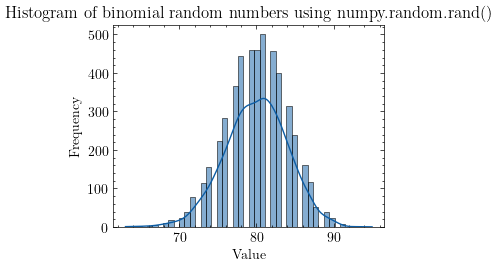
\includegraphics[scale=0.7]{imgs/binomialrv.png}  \\
            Time for generation: $0.0349$ seconds.
            Probability that $X < 50$: $0.00000000$.
            The theoretical answer for a Binomial Random Variable with ($n = 100, p = 0.8$) can be found by calculating
            % define the binomial distribution
            \begin{align*}
                P(X < 50) &= \sum_{k=0}^{49} {100 \choose k} (0.8)^k (0.2)^{100-k} \\
                &= 0.00000000
            \end{align*}

            which is approximately $0.00000000$.

        \item
            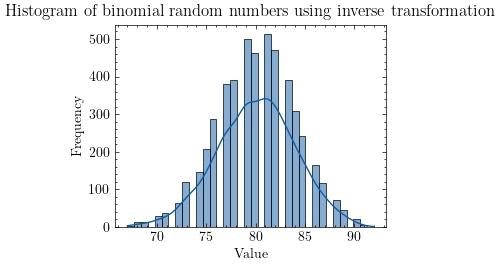
\includegraphics[scale=0.7]{imgs/binomialinverse.png}  \\
            Time for generation: $0.0350$ seconds.
        \item
            The histograms and the times for generation for the inverse method and NumPy's random number generator are
            very similar. The inverse method is slightly faster than NumPy's random number generator.
    \end{enumerate}

\section*{Question 4}
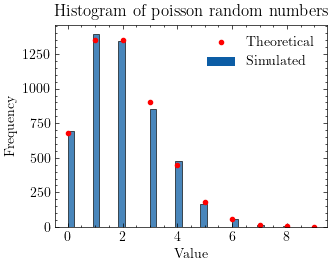
\includegraphics[scale=0.7]{imgs/poissonrv.png}  \\

\section*{Question 5}
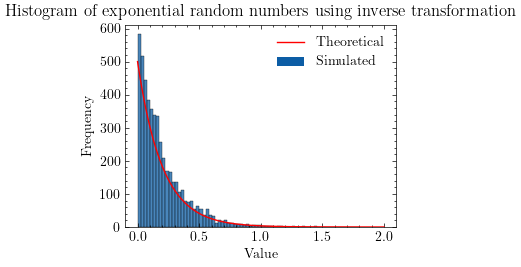
\includegraphics[scale=0.7]{imgs/exprv.png}  \\

\section*{Question 6}
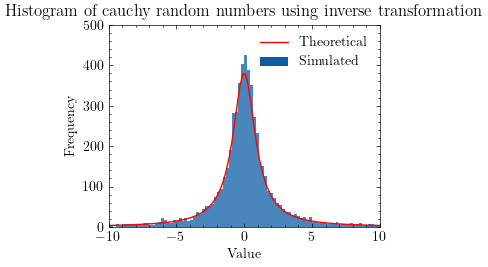
\includegraphics[scale=0.7]{imgs/cauchyrv.png}  \\

\section*{Question 7}
\begin{verbatim}
    n = 100
    n_sim = 10000
     
    # Run simulation
    hits = np.zeros(n_sim)
    for i in range(n_sim):
        deck = np.arange(1, n+1)
        np.random.shuffle(deck)
        hits[i] = np.sum(deck == np.arange(1, n+1))
        
    # Calculate expectation and variance
    print('Expectation:', np.mean(hits))
    print('Variance:', np.var(hits))
\end{verbatim}

With a repetition of $10000$ simulations, we find that the expectation is $1.0035$ and the variance is $1.01$.


We can calculate $\mathbb{E}[X]$ and $\mathbb{V}[X]$ exactly and compare them with our estimates. We have
\begin{align*}
    % expected value is 1
    \mathbb{E}[X] &= \sum_{i=1}^{100} i \cdot \frac{1}{100} = 1 \\
    % variance is 1
    \mathbb{V}[X] &= \sum_{i=1}^{100} (i - 1)^2 \cdot \frac{1}{100} - 1 = 1
\end{align*}

The estimates are very close to the exact values. This is expected because the number of simulations is large.

\section*{Question 8}
% A pair of fair dice are to be continually rolled until all the possible outcomes 2, 3, . . . , 12 have occurred at least
% once. Develop a simulation study to estimate the expected number of dice rolls that are needed.
\begin{verbatim}
    dice = np.arange(1, 7)
    n_sim = 10000
    
    # Run simulation
    rolls = np.zeros(n_sim)
    for i in range(n_sim):
        n_rolls = 0
        outcomes = np.zeros(11)
        while np.sum(outcomes == 0) > 0:
            roll = np.random.choice(dice, 2)
            n_rolls += 1
            outcomes[np.sum(roll) - 2] = 1
        rolls[i] = n_rolls
\end{verbatim}

We can model the number of rolls needed as a geometric random variable. We have
\[
    X \sim \text{Geometric}(p)
\]
where $p$ is the probability that all the possible outcomes have occurred at least once. We have
\[
    p = \frac{6 \cdot 5 \cdot 4 \cdot 3 \cdot 2 \cdot 1}{6^6} = \frac{720}{46656} \approx 0.0154
\]
We can then calculate the expected value of $X$ as
\[
    \mathbb{E}[X] = \frac{1}{p} = \frac{46656}{720} \approx 64.8
\]
The simulation gives us an estimate of $\mathbb{E}[X] \approx 64.8$. Then, the variance of $X$ is
\[
    \mathbb{V}[X] = \frac{1 - p}{p^2} = \frac{1 - 0.0154}{0.0154^2} \approx 4151.63
\]

\section*{Question 9}
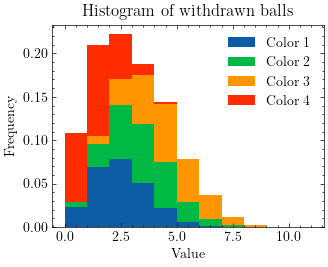
\includegraphics[scale=0.7]{imgs/balls.png}  \\
\begin{verbatim}
    n_sim = 10000
    n = 10
    balls = np.array([20, 30, 40, 10])

    # Run simulation
    x = np.zeros((n_sim, 4))
    for i in range(n_sim):
        urn = np.repeat(np.arange(4), balls)
        np.random.shuffle(urn)
        x[i] = np.bincount(urn[:n], minlength=4)
\end{verbatim}

\section*{Question 10}
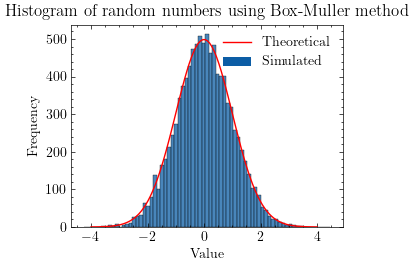
\includegraphics[scale=0.7]{imgs/boxmuller.png}  \\
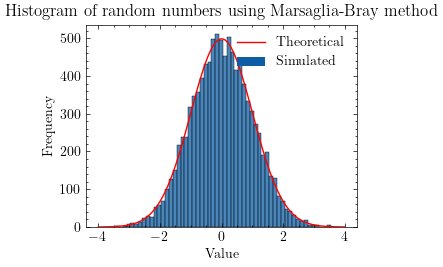
\includegraphics[scale=0.7]{imgs/marsagliabray.png}  \\
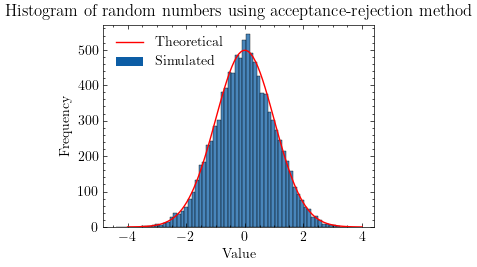
\includegraphics[scale=0.7]{imgs/acceptancerejection.png}  \\
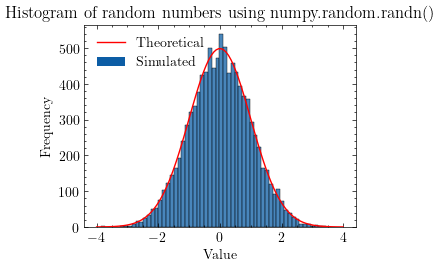
\includegraphics[scale=0.7]{imgs/numpyrandomrv.png}  \\

All of the methods seem to be very close to the theoereical normal distribution. 
\end{document}
